%
% Name Spaces of CafeOBJ
%
\documentclass[a4paper,oneside,10pt]{memoir}
\usepackage[hscale=0.76,vscale=0.76]{geometry}
\setlength{\parindent}{0.0cm}
\setlength{\parskip}{1.4ex}
\usepackage{graphicx}
\usepackage{proof}
\usepackage{fancyvrb}
%%% Japanese
%\usepackage{fontspec,xltxtra,xunicode}
%\usepackage{luatexja}
\usepackage{fontspec}
\usepackage{indentfirst}
\setmainfont[Mapping=tex-text]{M+ 2p medium}
\setsansfont[Mapping=tex-text]{M+ 2c}
\setmonofont[Mapping=tex-text]{M+ 2m medium}
\XeTeXlinebreaklocale "ja"
\XeTeXlinebreakskip=0em plus 0.1em minus 0.01em
\XeTeXlinebreakpenalty=0
\renewcommand{\baselinestretch}{1.4}
\settowidth{\parindent}{あ}
%%%%
\usepackage{dcolumn,hhline,colortbl}
\usepackage[table]{xcolor}
\usepackage{tikz}
\usetikzlibrary{shadows.blur,shapes,positioning,arrows.meta,arrows,decorations,calc}
%%%%% 色付表
\newcolumntype{G}{%
  >{\columncolor[gray]{0.9}}c}
\newcolumntype{O}{%
  >{\columncolor{orange}}c}
\newcolumntype{M}{%
  >{\columncolor{green}}c}
\newcolumntype{Y}{%
  >{\columncolor{yellow}}c}
\newcolumntype{C}{%
  >{\columncolor{cyan}}c}
%%%% hyperref
%\usepackage[dvipdfm,colorlinks=true,linkcolor=blue]{hyperref} 
\usepackage[colorlinks=true,linkcolor=blue]{hyperref} 
%%%%%%%%%%syntax
\makeatletter
% terminal - used for terminal symbols, argument is characters appear in sf.
\def\sym#1{\textsf{#1}\null}
% nonterm - used for non terminal symbols, argument is characters typed with
%           italic face.
\def\nonterm#1{\textit{#1}\null}
%%%%%
% syntax ... endsyntax
\def\xstrut{\relax\ifmmode\copy\strutbox\else\unhcopy\strutbox\fi}
\def\syntax{\syntaxoutnonbox\halign\bgroup
    \xstrut$\@lign##$\hfil &\hfil$\@lign{}##{}$\hfil
    &$\@lign##$\hfil &\qquad\@lign-- ##\hfil\cr}
\def\endsyntax{\crcr\egroup$$
  \global\@ignoretrue
}
\def\syntaxoutnonbox{\xleavevmode$$
    \parskip=0pt\lineskip=0pt
    \def\\{\crcr}% Must have \def and not \let for nested alignments.
    \everycr={\noalign{\penalty10000}}
    \tabskip=0pt}
\def\xleavevmode{\ifvmode\if@inlabel\indent\else\if@noskipsec\indent\else
    \if@nobreak\global\@nobreakfalse\everypar={}\fi
    {\parskip=0pt\noindent}\fi\fi\fi}
\def\@but{\noalign{\nointerlineskip}}
\def\alt{{\;|\;}}
\def\seqof#1{\mbox{\textbf{\{}}\;{#1}\;\mbox{\textbf{\}}}}
\def\optn#1{\textbf{[}\;{#1}\;\textbf{]}}
\def\synindent{\;\;\;}
\makeatother
%%%
%%%% numbering
%%% ToC down to susubsections
\settocdepth{subsubsection}
%%% Numbering down to sections
\setsecnumdepth{subsection}
%%% 名前定義を適当に
\def\figurename{{図}}
\def\tablename{表}
\def\contentsname{目次}
\def\listfigurename{図目次}
\def\listtablename{表目次}
\def\refname{参考文献}
\def\bibname{参考文献}
\def\indexname{索引}
\def\appendixname{付録}
%%%%%%%%%% Verbatim
\DefineVerbatimEnvironment%
{simplev}{Verbatim}
{fontsize=\small}
\DefineVerbatimEnvironment%
{examplev}{Verbatim}
{frame=leftline,fontsize=\small}
%%%%%%%%%%
\definecolor{shadecolor}{gray}{0.9}
\newenvironment{vvtm}%
{\parskip=0pt\lineskip=0pt\begin{center}\begin{minipage}{0.8\textwidth}\begin{snugshade}}%
  {\end{snugshade}\end{minipage}\end{center}}
%%%
\usepackage{float}
\begin{document}
\headstyles{default}
\tightlists
%\midsloppy
\sloppy
\raggedbottom
\chapterstyle{ell}
%%%%%%%%
\frontmatter
\pagestyle{empty}
% 表紙 %%%%%%%%%%%%%%%%%%%%%%%%%%%%%%%%%%%%%%%%%%%%%%%%%%%%%
\title{\textbf{CafeOBJ言語システムの名前空間}}
\author{澤田 寿実\\
  (株) 考作舎\\
  toshi.swd@gmail.com}
\date{}
\maketitle
 
\thispagestyle{empty}
\newpage
%%%%%%
\mainmatter
\pagestyle{plain}
\pagenumbering{arabic}
% 構成 %%%%%%%%%%%%%%%%%%%%%%%%%%%%%%%%%%%%%%%%%%%%%%%%%%%%%
\tableofcontents
\newpage
\chapter{CafeOBJ言語の名前空間と名前表示コマンド}
\label{chap:name-space}
CafeOBJ言語における「名前」,すなわち利用者が特定のオブジェクト\footnote{
本書ではCafeOBJ言語の利用者にとって中核をなすモノ(概念要素)をオブジェクトと呼ぶ.
厳密にはCaefOBJの形式的な構文定義に出現する各構文要素に対応してオブジェクトが%
存在し得るが,利用者が形式仕様を記述する上で理解しておくべき話とは無縁である.
知らなければならないのは,モジュール,オペレータ,ソート,公理,変数,パラメータ,%
それとモジュール式の解釈(それと--あれば--それらの属性)である.
従って本書ではこれのみを「オブジェクト」として参照する.
オブジェクトの中には「名前」によって参照出来ないものもある.}
を名付け,および参照するために使える文字列の構文規則について述べる.

続いて,モジュールの名前空間の表示コマンド,
および特定の名前を持ったオブジェクトの表示コマンドについて説明する.

\section{CafeOBJ言語の名前空間種別}
\label{sec:cafeobj-name-spaces}
本章ではCafeOBJ言語システムの名前空間の構造について調べる.
名前自身の構文については別途章を改める.

CafeOBJ言語の名前空間には次の2種がある:
\begin{enumerate}
\item トップレベル\\
  モジュール宣言とview宣言で導入された,それぞれモジュールおよびviewの名前の集合からなる.
\item モジュール\\
  ある特定のモジュールの中で参照可能な名前の集合であり,これは以下のものからなる:
  \begin{itemize}
    \item そのモジュールで宣言された以下のオブジェクトの名前:
      \begin{enumerate}
      \item パラメータの名前
      \item サブモジュールの名前
      \item ソートの名前
      \item オペレータの名前
      \item 変数の名前
      \item 公理ラベルの名前
      \end{enumerate}
    \item 輸入しているモジュールの名前空間に含まれる名前のうち,変数名を除いた名前
    \item トップレベルの名前空間に含まれる名前
  \end{itemize}
\end{enumerate}

以下これらの名前空間の構造について詳細を述べる.

\subsection{トップレベルの名前空間の構造と参照の解決}
\label{sec:toplevel-name-space}
上で述べた通りトップレベルの名前空間はモジュールの名前とviewの名前からなり,
これらは重なりを持つことがあり得る(図~\ref{fig:toplevel}を参照).

\begin{figure}[H]
\begin{center}
  \input toplevel.tikz
  %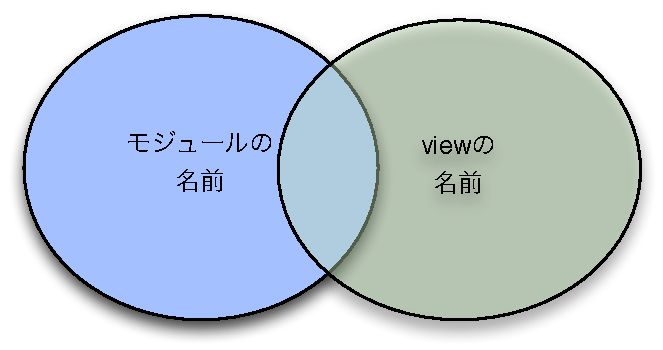
\includegraphics[scale=0.7]{toplevel.pdf}
\caption{トップレベルの名前空間}
\label{fig:toplevel}
\end{center}
\end{figure}

すなわち,同一の名前を持つモジュールとviewを宣言する事が可能である.
この場合モジュール式(第~\ref{sec:modexpr}章を参照)によっては
そこに出現する名前がモジュールの名前かviewの名前かで曖昧性が生ずる場合があり得るが,
本書が対象としているCafeOBJインタプリタでは以下のようにして曖昧さを回避する:
\begin{enumerate}
\item 指定の名前を持つviewを探す
\item その名前のviewが宣言されていれば,そのviewが指定されているものと解釈する
\item さもなければモジュールの名前が指定されているものと解釈する
\end{enumerate}

\subsection{モジュールの名前空間の構造と参照の解決}
\label{sec:inner-module-namaspece}

\subsubsection{サブモジュールを持たないモジュールの名前空間}
\label{sec:flat-module}

まず,輸入しているモジュール(サブモジュール)を持たないモジュールの名前空間の構造を%
図~\ref{fig:flat-module-namespece}に示す:
\begin{figure}[H]
\begin{center}
  \input flat-module.tikz
  %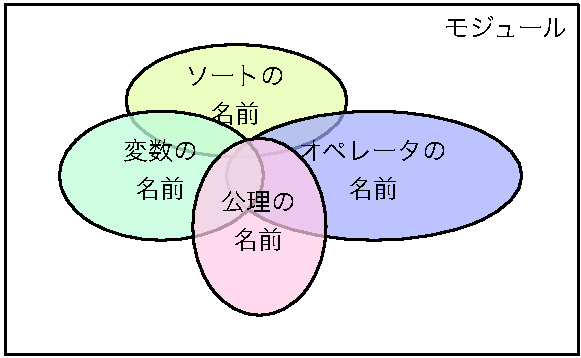
\includegraphics[scale=0.7]{flat-module.pdf}
\caption{サブモジュールなしのモジュールの名前空間}
\label{fig:flat-module-namespece}
\end{center}
\end{figure}
図から了解されるように,ソート,オペレータ,変数,公理それぞれで%
互いに同名のものが許される.
通常は名前の出現する文脈(構文)に応じてどの種のオブジェクトについての%
名前であるかが明確となるため曖昧性が生ずることは無い.
唯一あり得るのは,定数オペレータと変数の名前が同じ場合である.

\subsubsection{同名の定数項と変数の参照の解決}
まず,他のオペレータの引数に出現している場合 ``$f(N)$''を考える.
ここで名前 $N$ が定数オペレータ及び変数の名前として宣言されているとする.
システムは次のようにして項$f(N)$の解釈を試みる:
\begin{enumerate}
\item オペレータ$f$の引数のソートを調べる.たまたまこれが$S$であったとする.
\item $N$ という名前でかつソートが$S$以下の定数オペレータを探す.
\item これが見つかった場合$N$は定数オペレータの項であると解釈する.
\item 定数オペレータが見つからなかった場合は,$N$ という名前でソート$S$以下の変数を探す.
\item このような変数が見つかれば $N$ は変数項であると解釈する.
\item 上のいずれでもない場合は構文エラーとする.
\end{enumerate}
これで分かる通り,システムは項が出現する文脈に応じて期待されるソートにより%
制約をかけ,なおかつオペレータの名前の方を優先して解釈しようとする.
同名の変数と定数オペレータが互いに関係の無いソートのものであれば%
引数に出現する限りにおいて,曖昧性が生ずることは無い.

次に項 $N$ が単独で出現した場合であるが,これは解釈のための文脈がないため%
曖昧さを解消する術がない.
従ってこの場合は,項が曖昧であるとした構文エラーとして扱われる.

\subsubsection{階層的モジュールの名前空間の構造}
\label{sec:hierachical-module}
あるモジュールが他のモジュールを輸入している時,輸入されているモジュールを%
サブモジュールと呼ぶ.この時サブモジュールの名前空間に含まれる名前は,
\textbf{変数の名前を除いて}\footnote{
すなわち,輸入しているモジュールで宣言されている変数を参照することは出来ない.}
輸入しているモジュールの名前空間の一部となる(図~\ref{fig:hir-module}を参照).
図ではモジュールAがモジュールBを,モジュールBが%
モジュールCを輸入している場合が図示されている\footnote{一般にモジュールの輸入関係は%
有向グラフ構造となるが,ここでの議論に関して違いは無い.}.
\begin{figure}[!ht]
\begin{center}
  \input hir-module-namespace.tikz
  %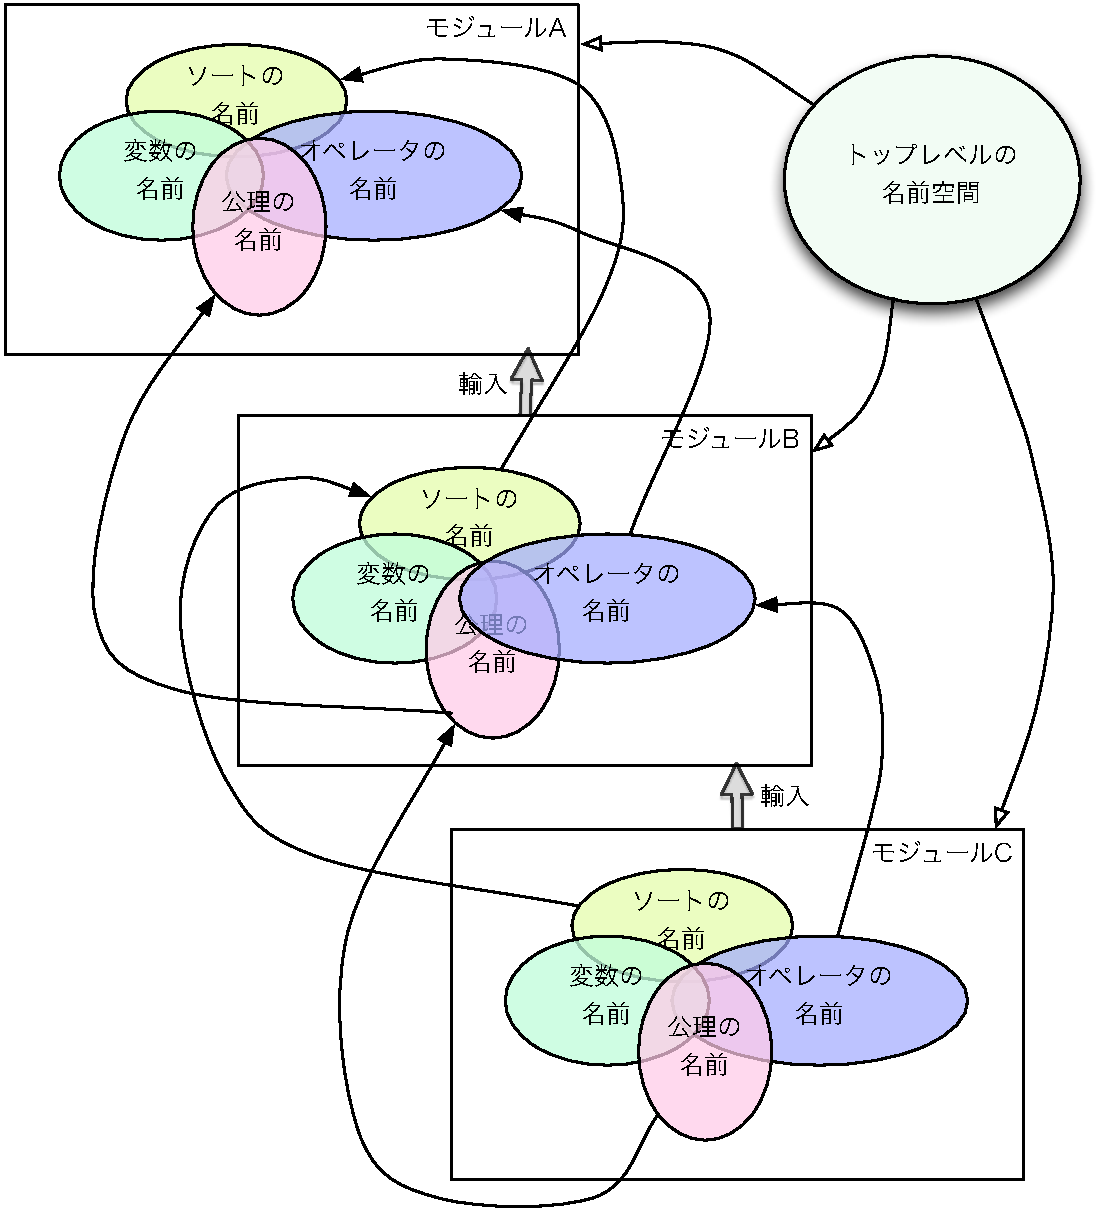
\includegraphics[scale=0.7]{hir-module-namespace.pdf}
  \caption{階層的モジュールの名前空間}
  \label{fig:hir-module}
\end{center}
\end{figure}

輸入されるサブモジュールはモジュール式と呼ばれる構文で指定される.
モジュールの名前はモジュール式の構成要素である.
モジュール式にはまた,viewの名前が含まれることがある\footnote{
モジュール式にはそこに含まれるモジュールの名前で参照されるモジュールの%
名前空間に含まれるソートやオペレータの名前も含む事が出来るが,
モジュール式の中で閉じたものであるため,ここではその詳細に触れない.}.
また,パラメータ付きモジュールのパラメータ宣言部にもモジュール式が出現する.
つまり,トップレベルの名前空間はモジュール宣言構文の一部(パラメータ宣言部及び%
モジュール輸入)において可視である.図にはその事も示されている.

\subsubsection{パラメータ}
パラメータもモジュール輸入の一形態と考えることが出来る\footnote{少なくとも%
名前空間と名前による参照を議論する場合,そのような解釈で問題ない.}.
すなわち,パラメータ $C :: M$ があった場合\footnote{$C$ はパラメータの名前,
$M$ はパラメータの仕様を規定するモジュール式.},
モジュール$M$の名前空間にある名前は,やはり(変数を除いて)%
そのパラメータを持つモジュールの名前空間の一部となる.
この場合,あたかも$C$という名前のモジュールが輸入されていると見なすことが出来る.

\subsubsection{文脈限定名による参照の曖昧性の解決}
\label{sec:qualified-name}
あるモジュール$A$がサブモジュールをもつ場合,
ある名前$\alpha$の参照が曖昧となる事があり得る.
\begin{figure}
\begin{center}
\input disunbig.tikz
%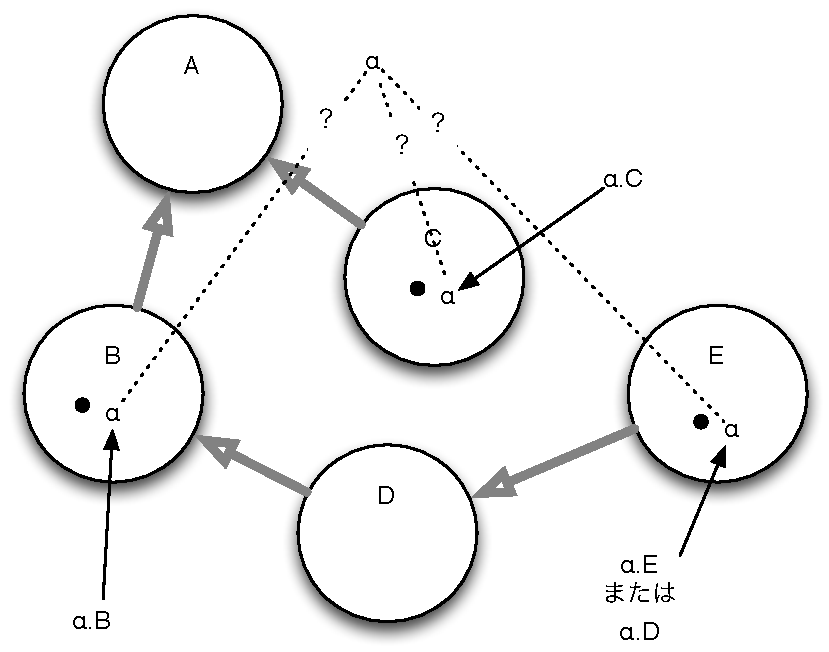
\includegraphics[scale=0.7]{disunbig.pdf}
\end{center}
\caption{名前の衝突と文脈限定名による解決}
\label{fig:disunbig}
\end{figure}
これらが互いに異なったオブジェクトの名前であれば特に問題は無い(変数と定数%
オペレータの名前の衝突については第~\ref{sec:flat-module}を参照).
しかし,例えば$\alpha$という名前が全てソートの名前だった場合,
構文上同じ文脈に登場することとなるため,%
どれを指し示すのかが曖昧である(図~\ref{fig:disunbig}を参照).
しかし名前の参照を解決する名前空間を制限すると,曖昧性が解消出来る.
例えば,図~\ref{fig:disunbig}のモジュールEの名前空間にある$\alpha$は,
モジュールDの名前空間では曖昧性が無い.
このような名前空間の制限に対する制限を指定する構文がCafeOBJにはあり,%
\textbf{文脈限定名}と呼ぶ.名前空間の指定にはモジュールの名前を用いる.
例えば名前$\alpha$についての文脈限定名は $\alpha.M$ の形式で表記され,$M$%
がモジュールの名前であり,\textbf{モジュール限定子}と呼ぶ.
名前$M$で示されるモジュールの名前空間で$\alpha$を解釈せよ,という意味となる.

文脈限定名$\alpha.M$ の$M$は,必ずしも参照対象とするオブジェクトの名前$\alpha$が%
導入されたモジュールの名前で無くとも良いことに注意されたい.
前述のように,サブモジュールの名前空間は(変数の名前を除き)輸入元の名前空間に
取り込まれるため,名前$\alpha$の参照について曖昧さが生じないような文脈でありさえすれば良い.

\subsubsection{文脈限定名が使える名前}
\label{sec:available-qualified-name}

全てのオブジェクトの名前について文脈限定名が使用出来るわけではなく,
使用可能なのは以下3つのオブジェクトのみである:
\begin{table}[htb]
\begin{vvtm}
\begin{center}
\begin{tabular}{l}
ソート \\
定数オペレータ \\
公理ラベル \\
\end{tabular}
\end{center}
\end{vvtm}
\caption{文脈限定名が使用可能なオブジェクト}
\label{tbl:qulifiable-names}
\end{table}

従ってこれら以外のオブジェクトで同名のものがある場合,曖昧性を解消する手段が無い.
そのような場合はモジュール式を用いて名前の付け替えを行い,
曖昧性を回避しなければならない.

%%%%%%%%%%%%%%%%%%%%%%%%%%%%%%%%%
\section{CafeOBJ言語の構文と名前}
\label{sec:cafeobj-syntax-and-names}
前章ではCafeOBJの名前空間について,CafeOBJの構文とは切り離して全体的な構造を調べた.
本章ではCafeOBJの言語の構文に基づいて,そこに出現する各種の「名前」について洗い出し,
構文上どこにどのような種類の「名前」が存在するかを確認する.

\subsection{構文表記法}
\label{sec:syntax-notation}
以下でCafeOBJの具体的な構文定義を参照するが,そこで使用される
表中構文は拡張BNF文法で定義されている.
生成規則の形式は次の通り:
\begin{syntax}
\synindent\synindent  nonterminal &::=& alternative \alt alternative \alt \cdots \alt alternative
\end{syntax}
これは,$nonterminal$ という構文要素は,$\alt$ で区切られた
それぞれの $alternative$ のどれかである事を意味する.

非終端シンボルは \textit{italic face} で,終端記号は
``\sym{terminal}'' のような字体で表記する.
また終端記号は `` と '' で囲み,拡張BNF文法で使用される
メタ文字と区別できるようにする事がある.
BNFの拡張形式は以下の通りである:
\begin{center}
\begin{minipage}{0.7\textwidth}
  \begin{tabular}{ll}
    a $\cdots$ & 1つ以上の a. \\
    a, $\cdots$ & カンマ記号で区分された一つ以上の\textit{a} のリスト: \\
    & ``a'' or ``a, a'' or ``a, a, a'', etc. \\
    $\seqof{\textrm{a}}$ & \textbf{\{} と \textbf{\}} はメタな構文括弧であり,これで囲まれた\\
    & \textit{a} はひとまとまりの構文カテゴリとして扱われる. \\
    $\optn{\textrm{a}}$ & \textit{a} はあっても無くとも良い: ``'' または ``a''.
  \end{tabular}
\end{minipage}
\end{center}
%%%%% 
\subsection{モジュール宣言の構文と名前}
\label{sec:module-decl}
以下にCafeOBJ言語のモジュール宣言の構文のうち「名前」に関係する部分について%
抜粋したものを示す.構文中 ``(1)'' のように先頭に番号が振っている構文規則が%
名前を含んでいるものである.
\begin{syntax}
(1)\  module &::=& module\_type\; module\_name \;
  \optn{parameters} \;
  \optn{principal\_sort} \\
  && \sym{``\{''}\; module\_elt\cdots \; \sym{``\}''} \\
  \synindent module\_type &::=& \sym{module} \alt \sym{module!} \alt
  \sym{module*}\\ 
  \synindent (2) module\_name &::=& ident \\
  parameters &::=& \sym{``(''}\; parameter, \cdots \sym{``)''}\\
  \synindent (3)\ parameter &::=&
  \optn{\sym{protecting}\alt\sym{extending}\alt\sym{including}}\; 
  paramter\_name \; 
  \sym{::}\; module\_expr \\
  \synindent (4)\ parameter\_name &::=& ident \\
  (5)\ principal\_sort &::=& \sym{principal-sort}\; sort\_name \\
  module\_elt &::=& import \alt sort  \alt operator \alt
  variable \alt axiom \alt macro \alt comment \\
  import &::=& \seqof{\sym{protecting}\alt\sym{extending}\alt\sym{including}\alt\sym{using}}
  \sym{``(''}\;module\_expr\;\sym{``)''}\\
  sort & ::= & visible\_sort \alt hidden\_sort \\
  \synindent visible\_sort & ::=& \sym{``[''}\; sort\_decl, \cdots \; \sym{``]''} \\
  \synindent hidden\_sort & ::=& \sym{``*[''}\; sort\_decl, \cdots \; \sym{``]*''} \\
  \synindent (6)\ sort\_decl &::=& sort\_name\; \cdots\; \optn{supersorts\; \cdots} \\
  \synindent (7)\ supersorts &::=& <\; sort\_name\; \cdots \\
  \synindent sort\_name &::=& sort\_symbol\optn{qualifier} 
  \\ 
  \synindent (8)\ sort\_symbol &::=& ident \\
  \synindent (9)\ qualifier &::=& \sym{``.''}module\_name\\
  (9)\ operator &::=& \seqof{\sym{op}\alt\sym{bop}}
               \; operator\_symbol\; : \; \optn{arity}\; \verb|->|\;
  coarity \; \optn{op\_attrs} \\
  \synindent (10)\ arity &::=& sort\_name \cdots \\
  \synindent (11)\ coarity &::=& sort\_name \\
  \synindent op\_attrs &::=& \sym{``\{''}\;op\_attr\cdots\;\sym{``\}''} \\
  (12)\ variable &::=& \sym{var}\; var\_name\; :\; sort\_name \alt
  \sym{vars} \; var\_name\cdots\; :\; sort\_name \\
  (13)\ \synindent var\_name &::=& ident \\
  axiom &::=& equation \alt cequation\alt transition \alt ctransition \alt fol\\
  \synindent equation &::=& \seqof{\sym{eq} \alt \sym{beq}}\;
  \optn{label}\; term \; \sym{=} \; term\; \sym{``.''}\\
  \synindent cequation &::=& \seqof{\sym{ceq} \alt \sym{bceq}}\;
  \optn{label}\; term \; \sym{=} 
  \; term\; \sym{if}\; term\;\sym{``.''} \\
  \synindent transition &::=& \seqof{\sym{trans} \alt \sym{btrans}}\;
  \optn{label}\; term \; \verb|=>| \; term \;\sym{``.''}\\
  \synindent ctransition &::=& \seqof{\sym{ctrans} \alt \sym{bctrans}}\;
  \optn{label}\; term \; \verb|=>| \; term\; \sym{if}\; term\;\sym{``.''}\\
  \synindent fol & ::= & \sym{ax} \optn{label}\; term \; \sym{``.''}\\
  \synindent (14)\ label &::=& \sym{``[''}\; label\_name\cdots\; \sym{``]:''}\\
  \synindent (15)\ label\_name &::=& ident\optn{qualifier} \\
\end{syntax}

\subsubsection{モジュール宣言文に出現する名前の種別}
\label{sec:names}
第~\ref{sec:module-decl}節で示した構文はCafeOBJ言語のモジュール宣言文の構文である.
ここにはCafeOBJ言語における「名前」のほとんど全て(view の名前を除く,これについては%
後述する)が出現している.前述のとおり,ここで示した構文定義中で ``(N)''のように%
番号をつけた構文で「名前」が出現している.
これらを整理すると以下の通りとなる.
これらの名前を使用することにより,利用者は対応するオブジェクトを参照する.

\begin{center}
  \begin{tabular}{@{} clll @{}}
    \toprule
    非終端記号 & 名前種別 & 参照先 & 構文番号\\ 
    \midrule
    $module\_name$ & モジュール名 & モジュール & (1)\\ 
    $parameter\_name$ & パラメータ名 &パラメータモジュール&(3) \\ 
    $sort\_name$ & ソート名 & ソート&(5),(6),(7),(10),(11)\\ 
    $operator\_symbol$ & オペレータ名 & オペレータ &(9)\\ 
    $var\_name$ & 変数名 & 変数&(12)\\ 
    $label\_name$ & 公理ラベル & 公理&(15) \\ 
    \bottomrule
  \end{tabular}
\end{center}

上に示した名前種別のうち,\nonterm{operator\_symbol}(オペレータ名)を除く全ての名前は%
CafeOBJ 言語の字句定義において \nonterm{ident}(識別子) として許される文字列により定義される%
\footnote{構文番号(2), (4) (8), (13), (14)を参照}.
構文(9)の\nonterm{qulifier}は第~\ref{sec:qualified-name}章で説明した%
文脈限定名を構成するモジュール限定子である.
第~\ref{sec:available-qualified-name}章では定数オペレータについても%
文脈限定名を使用する事が出来ると説明があったが,%
上記の構文定義中には反映されていない.
オペレータ名(\nonterm{operator\_symbol}については,
識別子(\nonterm{ident})と合わせて第~\ref{sec:token}章で説明する.

\subsection{モジュール式に出現する名前と名前空間}
\label{sec:modexpr}
下はモジュール式(\nonterm{module\_expr}の構文である.
\begin{syntax}
  module\_expr &::=& module\_name \alt sum \alt rename \alt instantiation 
  \alt \sym{``(''} module\_expr \sym{``)''} \\
  sum &::=& module\_expr\; \seqof{+\;\; module\_expr} \cdots \\
  rename &::=& module\_expr\;\sym{*}\;\sym{``\{''} rename\_map,\cdots
               \sym{``\}''} \\ 
  (1). instantiation &::=& module\_expr\;\sym{``(''}\textbf{\{}\;ident 
  [ qualifier ]\; \verb|<=|\; aview\textbf{\}},\;\cdots\;\sym{``)''}
  \\ 
  rename\_map &::=& sort\_map \alt op\_map \\
  (2). sort\_map &::=& \seqof{\sym{sort} \alt \sym{hsort}}\; 
  sort\_name \; \verb|->|\; ident \\
  (3). op\_map &::=& \seqof{\sym{op} \alt \sym{bop}}\;
                op\_name\;\verb|->|\;operaotr\_symbol \\
  (4). op\_name &::=& operator\_symbol\alt 
  \sym{``(''}operator\_symbol\sym{``)''}qualifier\\
  (5). aview &::=& view\_name\alt module\_expr\\
  & \alt & 
  \sym{view to}\; module\_expr\;\sym{``\{''} view\_elt,\cdots \sym{``\}''} \\
  (6). view\_name &::=& ident \\
  view\_elt &::=& sort\_map \alt op\_view \alt variable \\
  op\_view &::=& op\_map \alt term\; \verb|->|\; term
\end{syntax}


\subsection{view 宣言に出現する名前と名前空間}
\label{sec:view-declaration}

\begin{syntax}
  view &::=& \sym{view}\; view\_name\; \sym{from}\; module\_expr\; \sym{to}
  \; module\_expr \\
  && \sym{``\{''}\; view\_elt, \cdots \; \sym{``\}''} \\
\end{syntax}


\section{字句区切り文字と識別子,オペレータ名}
\label{sec:token}
識別子とオペレータ名はともに,不可視な文字を含まない連続したASCII英数字の文字列(\textbf{字句})
から構成される.
CafeOBJ システムは入力文字列を読み込む際に字句の区切りとして空白文字,タブ,改行,改ページ文字を
区切り記号として認識する.このような文字を\textbf{字句区切り文字}と呼ぶ.
すなわち,入力文字列は字句区切り文字によって切断される.
空白文字,タブ,改行,改ページのような不可視な文字は入力の際にスキップされ,
単なる字句の区切り記号として扱われる.これらに加えて以下の7文字が
字句区切り文字として定義されており,これらの文字はそれ自身で一つの字句を構成するものとして
認識される:
\begin{vvtm}
\begin{simplev}
   1. (          -- left paren 
   2. )          -- right paren
   3. [          -- left square bracket 
   4. ]          -- right square bracket
   5. {          -- left brace
   6. }          -- right brace
   7. ,          -- comma
\end{simplev}
\end{vvtm}

\subsection{識別子}
字句区切り文字は入力文字列から字句を切り出す印となる文字であるという性質上,
ソート名やモジュール名等の識別子を構成する文字として用いることは出来ない
\footnote{システムはこれらの文字を単純に自己自身で字句を構成する文字として読み込む.
そのため,文脈によってはエラーとならず,識別子を構成する文字として受け入れているように

見える場合がある.例えば``\texttt{[ \{SortName\} ]}''というソート宣言はエラーとならない.
しかし,実際にはこれは3つのソート ``\{'',``Sort'',``\}'' が宣言されたものとして認識される.}.

\subsection{オペレータ名}
一方,オペレータ名を構成する文字要素は上で述べた7つの可視な字句区切り文字のうち,%
1の丸括弧を除いてオペレータ名の一部として用いることが可能である%
\footnote{丸括弧はどの文脈においても``グルーピング''を表現するメタ文字として取り扱われる.}.
これらに加えて,空白文字もオペレータ名の一部として使用可能である.
例えば下は,''this is an operator'' という名前の2引数のオペレータの宣言である.
\begin{vvtm}
\begin{examplev}
module FOO {
  [ S ]
  op this is an operator : S S -> S
}
-- defining module FOO.._* done.
CafeOBJ> select FOO
FOO> sh op this       is an        operator 
.........................(this is an operator).........................
  * rank: S S -> S
  - attributes:  { prec: 0 }
FOO> 
\end{examplev}
\end{vvtm}
上の例を見て了解されるように,コマンドでオペレータ名を表記する際は%
オペレータ名を構成する連続した空白文字は無視され,1文字として扱われる.

また,mixfix オペレータの宣言において,項を表記する際の引き数位置を%
示すための下線(\verb|_|)はオペレータ名の一分として扱われる.
すなわち,コマンド類でオペレータを参照する際は下線(\verb|_|)も含めて%
指定する必要がある.コマンドの引数としてオペレータ名を指定する場合は%
次に示す例のように,下線(\verb|_|)とそれ以外の文字との間に空白文字を%
おいても良い.
\begin{vvtm}
\begin{simplev}
CafeOBJ> select NAT
NAT> sh op _+_
...............(_ + _) default attributes { assoc comm }...............
  * rank: NzNat NzNat -> NzNat
  - attributes:  { assoc comm demod prec: 33 r-assoc }
    - axioms:
      eq [:BDEMOD]: (NN:NzNat + NM:NzNat)
       = #! (+ nn nm)
      eq [:BDEMOD]: (M + N) = #! (+ m n)
  * rank: Nat Nat -> Nat
  - attributes:  { assoc comm idr: 0 demod prec: 33 r-assoc }
    - axioms:
      eq [:BDEMOD]: (AC:Nat + (NN:NzNat + NM:NzNat))
       = (AC + #! (+ nn nm))
      eq [:BDEMOD]: (M + N) = #! (+ m n)
      eq [ident1]: (0 + X-ID:Nat) = X-ID
NAT> sh op _ + _
...............(_ + _) default attributes { assoc comm }...............
  * rank: NzNat NzNat -> NzNat
  - attributes:  { assoc comm demod prec: 33 r-assoc }
    - axioms:
      eq [:BDEMOD]: (NN:NzNat + NM:NzNat)
       = #! (+ nn nm)
      eq [:BDEMOD]: (M + N) = #! (+ m n)
  * rank: Nat Nat -> Nat
  - attributes:  { assoc comm idr: 0 demod prec: 33 r-assoc }
    - axioms:
      eq [:BDEMOD]: (AC:Nat + (NN:NzNat + NM:NzNat))
       = (AC + #! (+ nn nm))
      eq [:BDEMOD]: (M + N) = #! (+ m n)
      eq [ident1]: (0 + X-ID:Nat) = X-ID
NAT> 
\end{simplev}
\end{vvtm}

\section{字句区切り文字の設定}
システムに組み込まれた字句区切り文字を追加するためのコマンドを新たに導入した.
本コマンドは新規の字句区切り文字の導入によるインパクトを評価するために用意したものであり,
将来的なCafeOBJ言語の字句区切り文字の拡張のための試験用に利用することを想定している.
\begin{vvtm}
\begin{simplev}
<Delimiterコマンド> ::= delimiter { + | - } "{" <文字> ... "}"
\end{simplev}
\end{vvtm}
\texttt{+}が指定された場合,\texttt{<文字>}で指定した文字を新たな字句など区切り文字として指定する.
逆に,新たに導入された字句区切り文字をキャンセルするには\texttt{-}を指定する.
本コマンドによって,システムに組み込みの字句区切り文字は影響を受けない(組み込みの字句区切り文字を
\texttt{-}指定によって字句区切り文字で無くすることは出来ない.

\section{モジュールの名前空間の表示}
\subsection{namesコマンド}
\label{sec:names-command}
今回新たに導入された \texttt{names} コマンドによって,
指定のモジュール内で可視の名前の一覧を見ることが出来る.
構文は下の通り:
\begin{vvtm}
\begin{simplev}
<名前表示コマンド>  ::= names [<モジュール式>] .
\end{simplev}
\end{vvtm}

\texttt{<モジュール式>}を省略すると,現在の文脈(モジュール)で%
可視の名前を表示する.
名前の表示はアルファベット順が原則であるが,
mixfix オペレータについては最後にまとめて表示される.

例: 下の例のモジュールFOOは組み込みモジュールのNATを輸入している.
その際に,ソートNatをNaturalに,ソート\_+\_ をplusと名前を付け替えている.
また,モジュール輸入構文で新たに導入された\texttt{as}指定によって%
\texttt{NAT *\{sort ....\}}のモジュールをNATURALという名前で参照できるように%
している.

\begin{vvtm}
\begin{examplev}
CafeOBJ> mod FOO { inc as NATURAL (NAT *{sort Nat -> Natural, op _+_ -> plus}) }
-- defining module FOO
; Loading /usr/local/cafeobj-1.4/lib/nat.bin
-- defining module! NAT
....
\end{examplev}
\end{vvtm}
上のモジュールFOOに対して\texttt{names}コマンドによって%
可視の名前を表示した結果を以下に示す.
\begin{vvtm}
\begin{examplev}
CafeOBJ> names FOO .

** [*] -----------------------------------------
*Cosmos*  
  - sort declared in CHAOS:UNIVERSAL
*HUniversal* 
  - hidden sort declared in CHAOS:UNIVERSAL
*Universal* 
  - sort declared in CHAOS:UNIVERSAL
** [:] -----------------------------------------
:BDEMOD   
  - axiom declared in NZNAT * { ... }
    eq [:BDEMOD]: (s NN:NzNat) = #! (1+ nn)
  - axiom declared in NZNAT * { ... }
    eq [:BDEMOD]: (NN:NzNat >= NM:NzNat)
     = #! (>= nn nm)
  - axiom declared in NZNAT * { ... }
    eq [:BDEMOD]: (NN:NzNat > NM:NzNat)
     = #! (> nn nm)
  - axiom declared in NZNAT * { ... }
    eq [:BDEMOD]: (NN:NzNat <= NM:NzNat)
     = #! (<= nn nm)
  - axiom declared in NZNAT * { ... }
    eq [:BDEMOD]: (NN:NzNat < NM:NzNat)
     = #! (< nn nm)
  - axiom declared in NZNAT * { ... }
    eq [:BDEMOD]: (NN:NzNat quot NM:NzNat)
     = #! (if (> nn nm) (truncate nn nm) 1)
  - axiom declared in NZNAT * { ... }
    eq [:BDEMOD]: (NN:NzNat * NM:NzNat)
     = #! (* nn nm)
  - axiom declared in NZNAT * { ... }
    eq [:BDEMOD]: d(NN:NzNat,NM:NzNat)
     = #! (if (= nn nm) 1 (abs (- nn nm)))
  - axiom declared in NZNAT * { ... }
    eq [:BDEMOD]: plus(NN:NzNat,NM:NzNat)
     = #! (+ nn nm)
  - axiom declared in NATURAL
    eq [:BDEMOD]: (p NN:NzNat) = #! (- nn 1)
  - axiom declared in NATURAL
    eq [:BDEMOD]: (s 0) = 1
  - axiom declared in NATURAL
    eq [:BDEMOD]: (N:Natural >= 0) = true
  - axiom declared in NATURAL
  \end{examplev}
  \end{vvtm}
  \begin{vvtm}
  \begin{examplev}
    eq [:BDEMOD]: (0 >= NN:NzNat) = false
  - axiom declared in NATURAL
    eq [:BDEMOD]: (NN:NzNat > 0) = true
  - axiom declared in NATURAL
    eq [:BDEMOD]: (0 > N:Natural) = false
  - axiom declared in NATURAL
    eq [:BDEMOD]: (0 <= N:Natural) = true
  - axiom declared in NATURAL
    eq [:BDEMOD]: (NN:NzNat <= 0) = false
  - axiom declared in NATURAL
    eq [:BDEMOD]: (0 < NN:NzNat) = true
  - axiom declared in NATURAL
    eq [:BDEMOD]: (N:Natural < 0) = false
  - axiom declared in NATURAL
    eq [:BDEMOD]: (NN:NzNat divides M:Natural)
     = #! (= 0 (rem m nn))
  - axiom declared in NATURAL
    eq [:BDEMOD]: (M:Natural rem NN:NzNat)
     = #! (rem m nn)
  - axiom declared in NATURAL
    eq [:BDEMOD]: (M:Natural quo NN:NzNat)
     = #! (truncate m nn)
  - axiom declared in NATURAL
    eq [:BDEMOD]: (N:Natural * 0) = 0
  - axiom declared in NATURAL
    eq [:BDEMOD]: plus(M:Natural,N:Natural)
     = #! (+ m n)
  - axiom declared in NATURAL
    eq [:BDEMOD]: sd(M:Natural,N:Natural)
     = #! (abs (- m n))
\end{examplev}
\end{vvtm}
\begin{vvtm}
\begin{examplev}
** [B] -----------------------------------------
BASE-BOOL 
  - indirect sub-module
BOOL      
  - indirect sub-module
Bool      
  - sort declared in TRUTH-VALUE
  - operator:
    op Bool : -> SortId { constr prec: 0 }
        -- declared in module TRUTH-VALUE
** [C] -----------------------------------------
CHAOS:PARSER 
  - indirect sub-module
CHAOS:UNIVERSAL 
  - indirect sub-module
** [D] -----------------------------------------
d         
  - operator:
    op d : NzNat NzNat -> NzNat { comm demod prec: 0 }
        -- declared in module NZNAT * { ... }
** [E] -----------------------------------------
EQL       
  - indirect sub-module
** [F] -----------------------------------------
false     
  - operator:
    op false : -> Bool { constr prec: 0 }
        -- declared in module TRUTH-VALUE
** [I] -----------------------------------------
ident0    
  - axiom declared in NZNAT * { ... }
    eq [ident0]: (1 * X-ID:NzNat) = X-ID
ident1    
  - axiom declared in NATURAL
    eq [ident1]: plus(0,X-ID:Natural)
     = X-ID
ident2    
  - axiom declared in NATURAL
    eq [ident2]: (1 * X-ID:Natural)
     = X-ID
\end{examplev}
\end{vvtm}
\begin{vvtm}
\begin{examplev}
** [N] -----------------------------------------
Natural   
  - sort declared in NAT-VALUE * { ... }
  - operator:
    op Natural : -> SortId { constr prec: 0 }
        -- declared in module NAT-VALUE * { ... }
NATURAL   
  - direct sub-module, alias of module NAT *{  ...  }
NzNat     
  - sort declared in NZNAT-VALUE
  - operator:
    op NzNat : -> SortId { constr prec: 0 }
        -- declared in module NZNAT-VALUE
NZNAT-VALUE 
  - indirect sub-module
** [P] -----------------------------------------
plus      
  - operator:
    op plus : Natural Natural -> Natural { assoc comm idr: 0 demod
                                           prec: 0 r-assoc }
        -- declared in module NATURAL
    op plus : NzNat NzNat -> NzNat { assoc comm demod prec: 0 r-assoc }
        -- declared in module NZNAT * { ... }
** [S] -----------------------------------------
sd        
  - operator:
    op sd : Natural Natural -> Natural { comm demod prec: 0 }
        -- declared in module NATURAL
SortId    
  - sort declared in CHAOS:PARSER
  - operator:
    op SortId : -> SortId { constr prec: 0 }
        -- declared in module CHAOS:PARSER
SyntaxErr 
  - sort declared in CHAOS:PARSER
  - operator:
    op SyntaxErr : -> SortId { constr prec: 0 }
        -- declared in module CHAOS:PARSER
\end{examplev}
\end{vvtm}
\begin{vvtm}
\begin{examplev}
** [T] -----------------------------------------
true      
  - operator:
    op true : -> Bool { constr prec: 0 }
        -- declared in module TRUTH-VALUE
TRUTH     
  - indirect sub-module
TRUTH-VALUE 
  - indirect sub-module
TypeErr   
  - sort declared in CHAOS:PARSER
  - operator:
    op TypeErr : -> SortId { constr prec: 0 }
        -- declared in module CHAOS:PARSER
** [Z] -----------------------------------------
Zero      
  - sort declared in NAT-VALUE * { ... }
  - operator:
    op Zero : -> SortId { constr prec: 0 }
        -- declared in module NAT-VALUE * { ... }
** [_] -----------------------------------------
_ Bottom _ 
  - sort declared in CHAOS:UNIVERSAL
_ HBottom _ 
  - hidden sort declared in CHAOS:UNIVERSAL
(if _ then _ else _ fi) 
  - operator:
    op if _ then _ else _ fi : Bool *Cosmos* *Cosmos* -> *Cosmos* { strat: (1 0)
                                                                    prec: 0
                                                                    }
        -- declared in module TRUTH
(not _)   
  - operator:
    op not _ : Bool -> Bool { strat: (0 1) prec: 53 }
        -- declared in module BASE-BOOL
(p _)     
  - operator:
    op p _ : NzNat -> Natural { demod prec: 15 }
        -- declared in module NATURAL
(parsed:[ _ ], rest:[ _ ]) 
  - operator:
    op parsed:[ _ ], rest:[ _ ] : *Universal* *Universal* -> SyntaxErr
                                  { prec: 0 }
        -- declared in module CHAOS:PARSER
\end{examplev}
\end{vvtm}
\begin{vvtm}
\begin{examplev}
(s _)     
  - operator:
    op s _ : NzNat -> NzNat { demod prec: 15 }
        -- declared in module NZNAT * { ... }
    op s _ : Natural -> NzNat { demod prec: 15 }
        -- declared in module NATURAL
(_ * _)   
  - operator:
    op _ * _ : NzNat NzNat -> NzNat { assoc comm idr: 1 demod prec: 31
                                      r-assoc }
        -- declared in module NZNAT * { ... }
    op _ * _ : Natural Natural -> Natural { assoc comm idr: 1 demod
                                            prec: 31 r-assoc }
        -- declared in module NATURAL
(_ := _)  
  - operator:
    pred _ := _ : *Cosmos* *Cosmos*  { prec: 51 }
        -- declared in module TRUTH
(_ :is _) 
  - operator:
    pred _ :is _ : *Cosmos* SortId  { prec: 125 }
        -- declared in module TRUTH
(_ < _)   
  - operator:
    pred _ < _ : NzNat NzNat  { demod prec: 51 }
        -- declared in module NZNAT * { ... }
    pred _ < _ : Natural Natural  { demod prec: 51 }
        -- declared in module NATURAL
(_ <= _)  
  - operator:
    pred _ <= _ : NzNat NzNat  { demod prec: 51 }
        -- declared in module NZNAT * { ... }
    pred _ <= _ : Natural Natural  { demod prec: 51 }
        -- declared in module NATURAL
(_ = _)   
  - operator:
    pred _ = _ : *Cosmos* *Cosmos*  { comm prec: 51 }
        -- declared in module EQL
\end{examplev}
\end{vvtm}
\begin{vvtm}
\begin{examplev}
(_ =*= _) 
  - operator:
    pred _ =*= _ : *HUniversal* *HUniversal*  { prec: 51 }
        -- declared in module TRUTH
(_ =/= _) 
  - operator:
    pred _ =/= _ : *Cosmos* *Cosmos*  { prec: 51 }
        -- declared in module TRUTH
(_ == _)  
  - operator:
    pred _ == _ : *Cosmos* *Cosmos*  { prec: 51 }
        -- declared in module TRUTH
(_ =b= _) 
  - operator:
    pred _ =b= _ : *Cosmos* *Cosmos*  { prec: 51 }
        -- declared in module TRUTH
(_ > _)   
  - operator:
    pred _ > _ : NzNat NzNat  { demod prec: 51 }
        -- declared in module NZNAT * { ... }
    pred _ > _ : Natural Natural  { demod prec: 51 }
        -- declared in module NATURAL
(_ >= _)  
  - operator:
    pred _ >= _ : NzNat NzNat  { demod prec: 51 }
        -- declared in module NZNAT * { ... }
    pred _ >= _ : Natural Natural  { demod prec: 51 }
        -- declared in module NATURAL
(_ and _) 
  - operator:
    op _ and _ : Bool Bool -> Bool { assoc comm prec: 55 r-assoc }
        -- declared in module BASE-BOOL
(_ and-also _) 
  - operator:
    op _ and-also _ : Bool Bool -> Bool { strat: (1 0 2) prec: 55
                                          r-assoc }
        -- declared in module BASE-BOOL
\end{examplev}
\end{vvtm}
\begin{vvtm}
\begin{examplev}
(_ divides _) 
  - operator:
    pred _ divides _ : NzNat Natural  { demod prec: 51 }
        -- declared in module NATURAL
(_ iff _) 
  - operator:
    op _ iff _ : Bool Bool -> Bool { strat: (0 1 2) prec: 63 r-assoc }
        -- declared in module BASE-BOOL
(_ implies _) 
  - operator:
    op _ implies _ : Bool Bool -> Bool { strat: (0 1 2) prec: 61
                                         r-assoc }
        -- declared in module BASE-BOOL
(_ or _)  
  - operator:
    op _ or _ : Bool Bool -> Bool { assoc comm prec: 59 r-assoc }
        -- declared in module BASE-BOOL
(_ or-else _) 
  - operator:
    op _ or-else _ : Bool Bool -> Bool { strat: (1 0 2) prec: 59
                                         r-assoc }
        -- declared in module BASE-BOOL
(_ quo _) 
  - operator:
    op _ quo _ : Natural NzNat -> Natural { demod prec: 41 }
        -- declared in module NATURAL
(_ quot _) 
  - operator:
    op _ quot _ : NzNat NzNat -> NzNat { demod prec: 31 l-assoc }
        -- declared in module NZNAT * { ... }
(_ rem _) 
  - operator:
    op _ rem _ : Natural NzNat -> Natural { demod prec: 31 l-assoc }
        -- declared in module NATURAL
(_ xor _) 
  - operator:
    op _ xor _ : Bool Bool -> Bool { assoc comm prec: 57 r-assoc }
        -- declared in module BASE-BOOL
CafeOBJ> 
\end{examplev}
\end{vvtm}

\subsection{look up コマンド}
\label{sec:lookup-command}
\texttt{look up} コマンドは,指定のあるいは現在文脈のモジュールにおいて,%
ある名前で参照されるものが何であるかを表示する.
構文は次の通りである.
\begin{vvtm}
\begin{simplev}
<LOOK UPコマンド>    ::= lookup [in <モジュール名> :] <識別子> | <オペレータ名> .
\end{simplev}
\end{vvtm}
例:この例は,先に第~\ref{sec:names-command}章で見たモジュールFOO内で%
\texttt{plus}という名前で参照されるものが何であるかを表示したものである.
\begin{vvtm}
\begin{simplev}
CafeOBJ> look up in FOO : plus .

** [P] -----------------------------------------
plus      
  - operator:
    op plus : Natural Natural -> Natural { assoc comm idr: 0 demod
                                           prec: 0 r-assoc }
        -- declared in module NATURAL
    op plus : NzNat NzNat -> NzNat { assoc comm demod prec: 0 r-assoc }
        -- declared in module NZNAT * { ... }
CafeOBJ> select FOO
FOO> look up Natural
.

** [N] -----------------------------------------
Natural   
  - sort declared in NAT-VALUE * { ... }
  - operator:
    op Natural : -> SortId { constr prec: 0 }
        -- declared in module NAT-VALUE * { ... }
FOO> 
\end{simplev}
\end{vvtm}

\end{document}


%%% Local Variables:
%%% mode: latex
%%% TeX-master: t
%%% End:
